\clearpage
\newpage

\section{Problem 3 (22 pts)}

\subsection{Part 1}
\begin{enumerate}
    \item Visualize all models of behavior.
    \begin{figure}[hbt!]
        \centering
        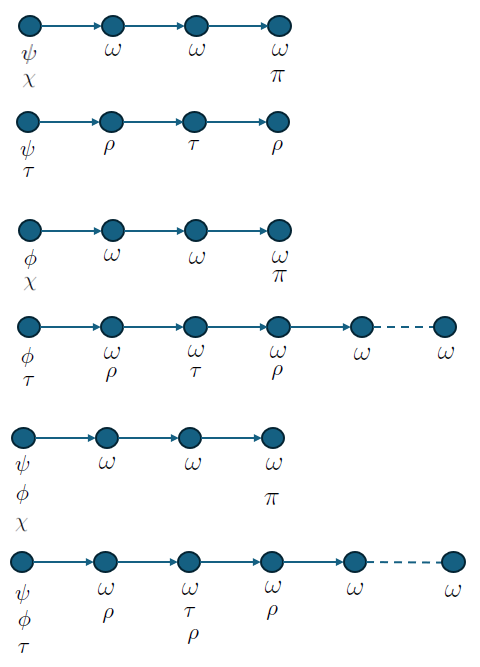
\includegraphics[scale=0.6]{assigment1/331A1_num3_part1.png}
        \caption{Models of behavior for Problem 3.1.1}
        \label{fig:model_behavior}
    \end{figure}

    \item Make observations on the visualization by specifying exact conditions about
termination, non-termination and consistency (or lack thereof), if any exist.\\

\textbf{Termination: } A you can see with the image above, we have some models that will terminate. For example, the first one will terminate because as soon as $\pi$ is true, the other condition ($\pi\mathcal{R}\omega$) will stop.\\ \\
\textbf{Non-termination: } The examples 4 and 6 represent non-termination models since $\omega$ will stay true until and including the state at which $\pi$ first becomes true.\\ \\
\textbf{Consistency: } They are not paths that are consistent with the temporal formula. The closest one is the last one that adheres to 6 out of the 7 of the temporal constraints.\\ \\

\end{enumerate}

\subsection{Part 2}
\begin{enumerate}
    \item Formalize and visualize the following requirement: “If none of ϕ or ψ are
invariants, then starting from time = i + 2, χ will eventually become true and it will
remain true up to and including the moment τ first becomes true. Note that there
exists no guarantee that τ ever becomes true.”
    \begin{figure}[hbt!]
        \centering
        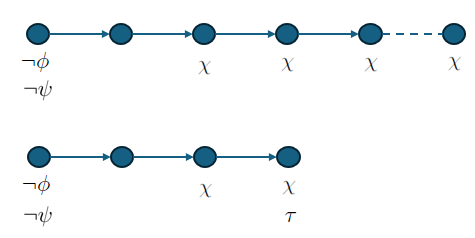
\includegraphics[scale=0.58]{assigment1/331A1_num3_part2.1.png}
        \caption{Models of behavior for Problem 3.2.1}
        \label{fig:model_behavior}
    \end{figure}

\begin{lstlsting}

This requirement can be formalize as follows:\[
    (\neg\phi \vee \neg\psi) \rightarrow \bigcirc^2(\Box \chi \land (\chi \mathcal{U} \tau))
    \]

    \item Describe the visualize the following requirement: \[
    (\neg\alpha \vee \neg\beta) \rightarrow (\bigcirc\diamond(\gamma \mathcal{U} \delta))
    \]

($\neg \alpha \land \neg \beta$) signifies that either $\alpha$ is not true, or  $\beta$ is not true, or both are not true. $(\bigcirc\diamond(\gamma \mathcal{U} \delta))$ means that there will eventually be a time from which point forward ($\Box$) it will always be the case that $\gamma$ holds until $\delta$ becomes true. Note that in this case, $\delta$ is guaranteed to become true at some future time. This is the definition of the $\mathcal{U}$ operation.
    \begin{figure}[hbt!]
        \centering
        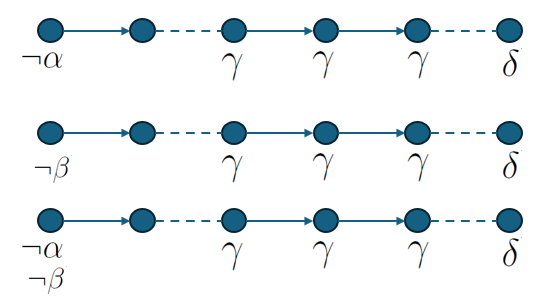
\includegraphics[scale=0.5]{assigment1/331A1_num3_part2.2.png}
        \caption{Models of behavior for Problem 3.2.2}
        \label{fig:model_behavior}
    \end{figure}

    \item Describe the visualize the following requirement: \[
    (\bigcirc \tau \land \bigcirc \Box \Diamond \chi) \rightarrow \bigcirc^2 (\phi \mathcal{W} \psi)
    \]
This requirement signifies that at iteration \textit{i + 1} $\tau$ will become true and eventually $\chi$ will always be true (not necessarily at \textit{i + 1}). At \textit{i + 2} $\psi$ will be true until $\phi$ becomes true.
    \begin{figure}[hbt!]
        \centering
        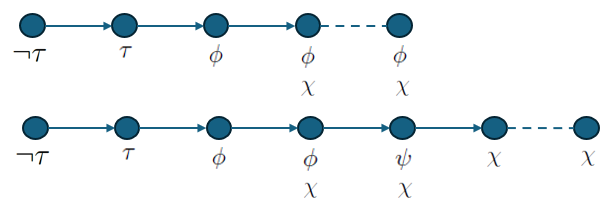
\includegraphics[scale=0.5]{assigment1/331A1_num3_part2.3.png}
        \caption{Models of behavior for Problem 3.2.3}
        \label{fig:model_behavior}\\
    \end{figure}

\end{enumerate}
